\documentclass[conference]{IEEEtran}
\usepackage{times}
\usepackage{amsmath,amssymb,amsfonts}
\usepackage{graphicx}
\usepackage{textcomp}
\usepackage{xcolor}
\usepackage{booktabs}
\usepackage{hyperref}
\usepackage{url}
\usepackage{multirow}
\usepackage{subcaption}
\usepackage[T1]{fontenc}

\def\BibTeX{{\rm B\kern-.05em{\sc i\kern-.025em b}\kern-.08em T\kern-.1667em\lower.7ex\hbox{E}\kern-.125emX}}

\begin{document}

\title{TLabel: A Unified Annotation Framework for\\Cross-Sensor Tactile Manipulation Data}

\author{\IEEEauthorblockN{Xi Luo}
\IEEEauthorblockA{Niuxu Tech\\
Hangzhou, China\\
xi.luo@niuxutech.com}}

\maketitle

\begin{abstract}
Code and schema: \url{https://github.com/liesliy/tlabel}

Tactile datasets today ship as raw sensor signals---video frames, HDF5 arrays, custom blobs---without semantic annotations that describe what is happening in contact, force, or slip terms. Each sensor type demands its own ad-hoc processing, and results from different sensors cannot be compared or fused. We introduce TLabel Format, the first cross-sensor tactile annotation schema with capability declarations: each sensor adapter explicitly declares which of ten semantic dimensions it can and cannot annotate, and only outputs supported fields. This mechanism enables heterogeneous sensors---regardless of operating principle---to produce compatible annotations while preserving their unique strengths. We validate TLabel on two sensors with fundamentally different physics: Daimon-Infinity (vision-based GelSight, 94 episodes, 6 tasks) and PaXini PXCap (6D Hall-effect distributed array, 15 episodes, 7 tasks). Both adapters achieve zero hard errors across 590K+ observations. Unlike prior work that unifies tactile representations at the raw-signal or learned-feature level (T3, AnyTouch, SITR), TLabel unifies at the semantic annotation level, producing structured labels that are directly consumable by downstream models without retraining. Downstream evaluation confirms measurable benefits: +7.93\% cross-scenario generalization accuracy and +10.35\% slip-risk F1. Our results show that cross-sensor tactile annotation is feasible, that the two dominant sensing paradigms---vision-based and distributed array---are complementary rather than competing, and that capability declarations provide a practical mechanism for managing sensor heterogeneity.
\end{abstract}

\begin{IEEEkeywords}
tactile sensing, cross-sensor annotation, data standardization, manipulation, capability declaration
\end{IEEEkeywords}

\section{Introduction}

Tactile sensing enables robots to perceive contact, force, and slip during manipulation---capabilities essential for tasks ranging from precision assembly to delicate object handling. Recent years have seen a proliferation of tactile sensor designs: vision-based sensors (e.g., GelSight, DIGIT) that capture surface deformation at high spatial resolution, and distributed taxel arrays (e.g., PaXini PXCap, tactile gloves) that measure force distribution across the entire hand.

Despite this hardware diversity, a fundamental gap remains: \textbf{there is no standardized way to annotate tactile data}. Each dataset ships in its own format---raw video frames, HDF5 arrays, or custom binary blobs---without semantic labels that describe \emph{what is happening} in tactile terms. This creates three concrete problems:

\begin{enumerate}
\item \textbf{Data remains silent.} Most tactile datasets contain rich contact information, but without structured annotations, this information cannot be directly used for training contact-aware policies or safety monitors.
\item \textbf{Methods are not reusable.} Annotation approaches developed for one sensor type (e.g., optical flow for GelSight) cannot be applied to another (e.g., force thresholding for taxel arrays), forcing redundant development.
\item \textbf{Cross-sensor comparison is impossible.} Without a shared annotation vocabulary, researchers cannot compare tactile phenomena across sensor modalities or fuse annotations from heterogeneous sources.
\end{enumerate}

We address these challenges with \textbf{TLabel Format}, the first cross-sensor tactile annotation schema that uses capability declarations to manage sensor heterogeneity. The key insight is that while raw tactile signals differ fundamentally across sensor types (images vs.\ force vectors), the \emph{semantic phenomena} they capture---contact, force, slip, manipulation phases---are shared. TLabel operates at this semantic level: each sensor adapter declares which of ten semantic dimensions it can and cannot annotate (e.g., slip direction, texture, whole-hand coordination), and the annotation layer only outputs supported fields. This allows different sensors to share the same output format while preserving their unique strengths.

Unlike prior cross-sensor work that unifies at the representation level---T3~\cite{zhao2024t3} uses sensor-specific encoders with shared trunks, AnyTouch~\cite{feng2025anytouch} aligns tactile-textual features, and SITR~\cite{sitr2025} learns sensor-invariant embeddings via simulation---TLabel unifies at the \emph{semantic annotation} level. This is a complementary layer: representation learning produces embeddings for model training, while TLabel produces structured labels that are directly interpretable, comparable across sensors, and consumable by downstream tasks without retraining.

We validate TLabel through two independent adapters for sensors with fundamentally different operating principles:
\begin{itemize}
\item \textbf{Daimon-Infinity adapter} for vision-based GelSight sensors (image$\rightarrow$pixel deviation$\rightarrow$annotation)
\item \textbf{PaXini adapter} for 6D Hall-effect distributed taxel arrays (numeric vectors$\rightarrow$force thresholds$\rightarrow$annotation)
\end{itemize}

Our contributions are:
\begin{enumerate}
\item \textbf{TLabel Format}, the first cross-sensor tactile annotation schema with capability declarations, enabling heterogeneous sensors to produce compatible semantic annotations while preserving their unique strengths
\item Two validated adapters covering the two dominant tactile sensing paradigms---vision-based (GelSight) and distributed array (6D Hall-effect)---demonstrating that sensors with fundamentally different physics can share a unified annotation output
\item Systematic quality validation across 109 episodes and 590K+ observations: zero hard errors in both adapters, with anomaly rates of 2.91\% (GelSight) and 0.14\% (6D Hall)
\item Downstream evidence that semantic annotations provide measurable benefits: +7.93\% cross-scenario generalization ($p<0.01$) and +10.35\% slip-risk F1, confirming that structured labels are not merely consistent but useful
\end{enumerate}

\section{Related Work}

\subsection{Tactile Datasets and Annotation}

The tactile sensing community has produced datasets of growing scale and diversity. Daimon-Infinity~\cite{daimon2026} provides 10,000+ hours of vision-tactile-language-action data with 114-dimensional observations, but its annotations focus on task-level labels (object category, skill type) rather than per-frame tactile semantics. FoTa~\cite{fota2024} aggregates 3.08M samples across 13 sensor types for unified training, yet lacks structured tactile annotations. TacQuad~\cite{tacquad2025} offers paired multi-sensor data with text descriptions generated by GPT-4o, and OpenTouch~\cite{opentouch2025} uses GPT-5 for automatic annotation at $\sim$90\% accuracy---but these are object-level descriptions, not frame-level tactile phenomena.

A critical gap persists: \textbf{no existing dataset provides standardized per-frame tactile annotations} (contact state, force level, slip events) that are comparable across sensor types. Each dataset uses its own ad-hoc labeling, making cross-dataset analysis impossible.

\subsection{Cross-Sensor Tactile Representation}

Several works address sensor heterogeneity at the representation level. T3~\cite{zhao2024t3} employs sensor-specific encoders with a shared trunk, enabling zero-shot transfer across sensors through transferable tactile transformers. AnyTouch~\cite{feng2025anytouch} introduces a multi-level representation framework combining masked image modeling with text-aligned cross-sensor matching. SITR~\cite{sitr2025} uses physically-based rendering to simulate 100 sensor configurations for zero-shot sensor-invariant representations. TLV-CoRe~\cite{tlvcore2025} aligns tactile, language, and vision through a sensor-aware modulator.

These works unify representations at the \emph{raw signal} or \emph{learned feature} level. TLabel complements this by unifying at the \emph{semantic annotation} level---providing structured labels that are directly interpretable and usable for downstream tasks, regardless of the underlying sensor type.

\subsection{Contact, Force, and Slip Detection}

Contact and slip detection from tactile signals has been extensively studied for vision-based sensors. Dong et al.~\cite{dong2017gelsight} established that marker displacement fields on GelSight surfaces correlate linearly with normal and shear forces, and that displacement field entropy characterizes partial slip---a method adopted in our GelSight adapter. Hu et al.~\cite{hu2024slip} extended this with contact force field entropy analysis, achieving 95.6\% slip detection accuracy without object priors. FeelAnyForce~\cite{feelanyforce2025} uses multi-head Transformers for force estimation across unseen objects, and FEATS~\cite{feats2024} generates force labels via finite element analysis.

For distributed taxel arrays, contact detection typically relies on threshold-based methods~\cite{paxini2025}, and slip is inferred indirectly from pressure distribution changes rather than direct shear measurement. The Sparsh benchmark~\cite{sparsh2024} defines six downstream tasks including force estimation and slip detection, but focuses on evaluation rather than annotation standardization.

TLabel draws on these methods as adapter-level implementations while abstracting their outputs into a sensor-agnostic format.

\subsection{Embodied AI Data Standards}

Standardization efforts in embodied AI have largely overlooked tactile data. Open X-Embodiment~\cite{openx2024} defines RLDS format for 22 robot platforms with vision and proprioception, but includes \textbf{no tactile annotation schema}. LeRobot~\cite{lerobot2024} provides HDF5-based data storage with optional observation extensions, but \textbf{lacks standardized tactile annotation fields}. ROS2 offers custom message types for tactile data (PointCloud2, ContactsState) without a unified semantic specification.

This standardization gap is precisely where TLabel operates: defining what tactile annotations \emph{should look like} rather than how raw signals are stored.

\section{TLabel Format}

\subsection{Design Principles}

TLabel Format is designed around three principles:

\textbf{Sensor-agnostic output.} All annotations are expressed in terms of semantic tactile concepts (contact state, force level, slip, manipulation phase) rather than raw sensor signals. This decouples downstream consumers from sensor-specific details.

\textbf{Capability declarations.} Not all sensors can annotate all dimensions---a GelSight sensor can detect slip direction and texture, while a distributed array cannot; conversely, a distributed array provides whole-hand coordination that a fingertip-only sensor cannot. TLabel uses a \texttt{capabilities} dictionary to declare support for 10 semantic dimensions, and adapters only output fields they support.

\textbf{Extensibility.} New sensor types can be added by implementing an adapter that reads their raw data and outputs TLabel Format JSON. The schema version field allows backward-compatible evolution.

\subsection{Schema Structure}

Fig.~\ref{fig:architecture} shows the overall architecture. Raw sensor data from heterogeneous sources is processed by sensor-specific adapters, each declaring its capabilities and producing a unified JSON output.

\begin{figure}[t]
\centering
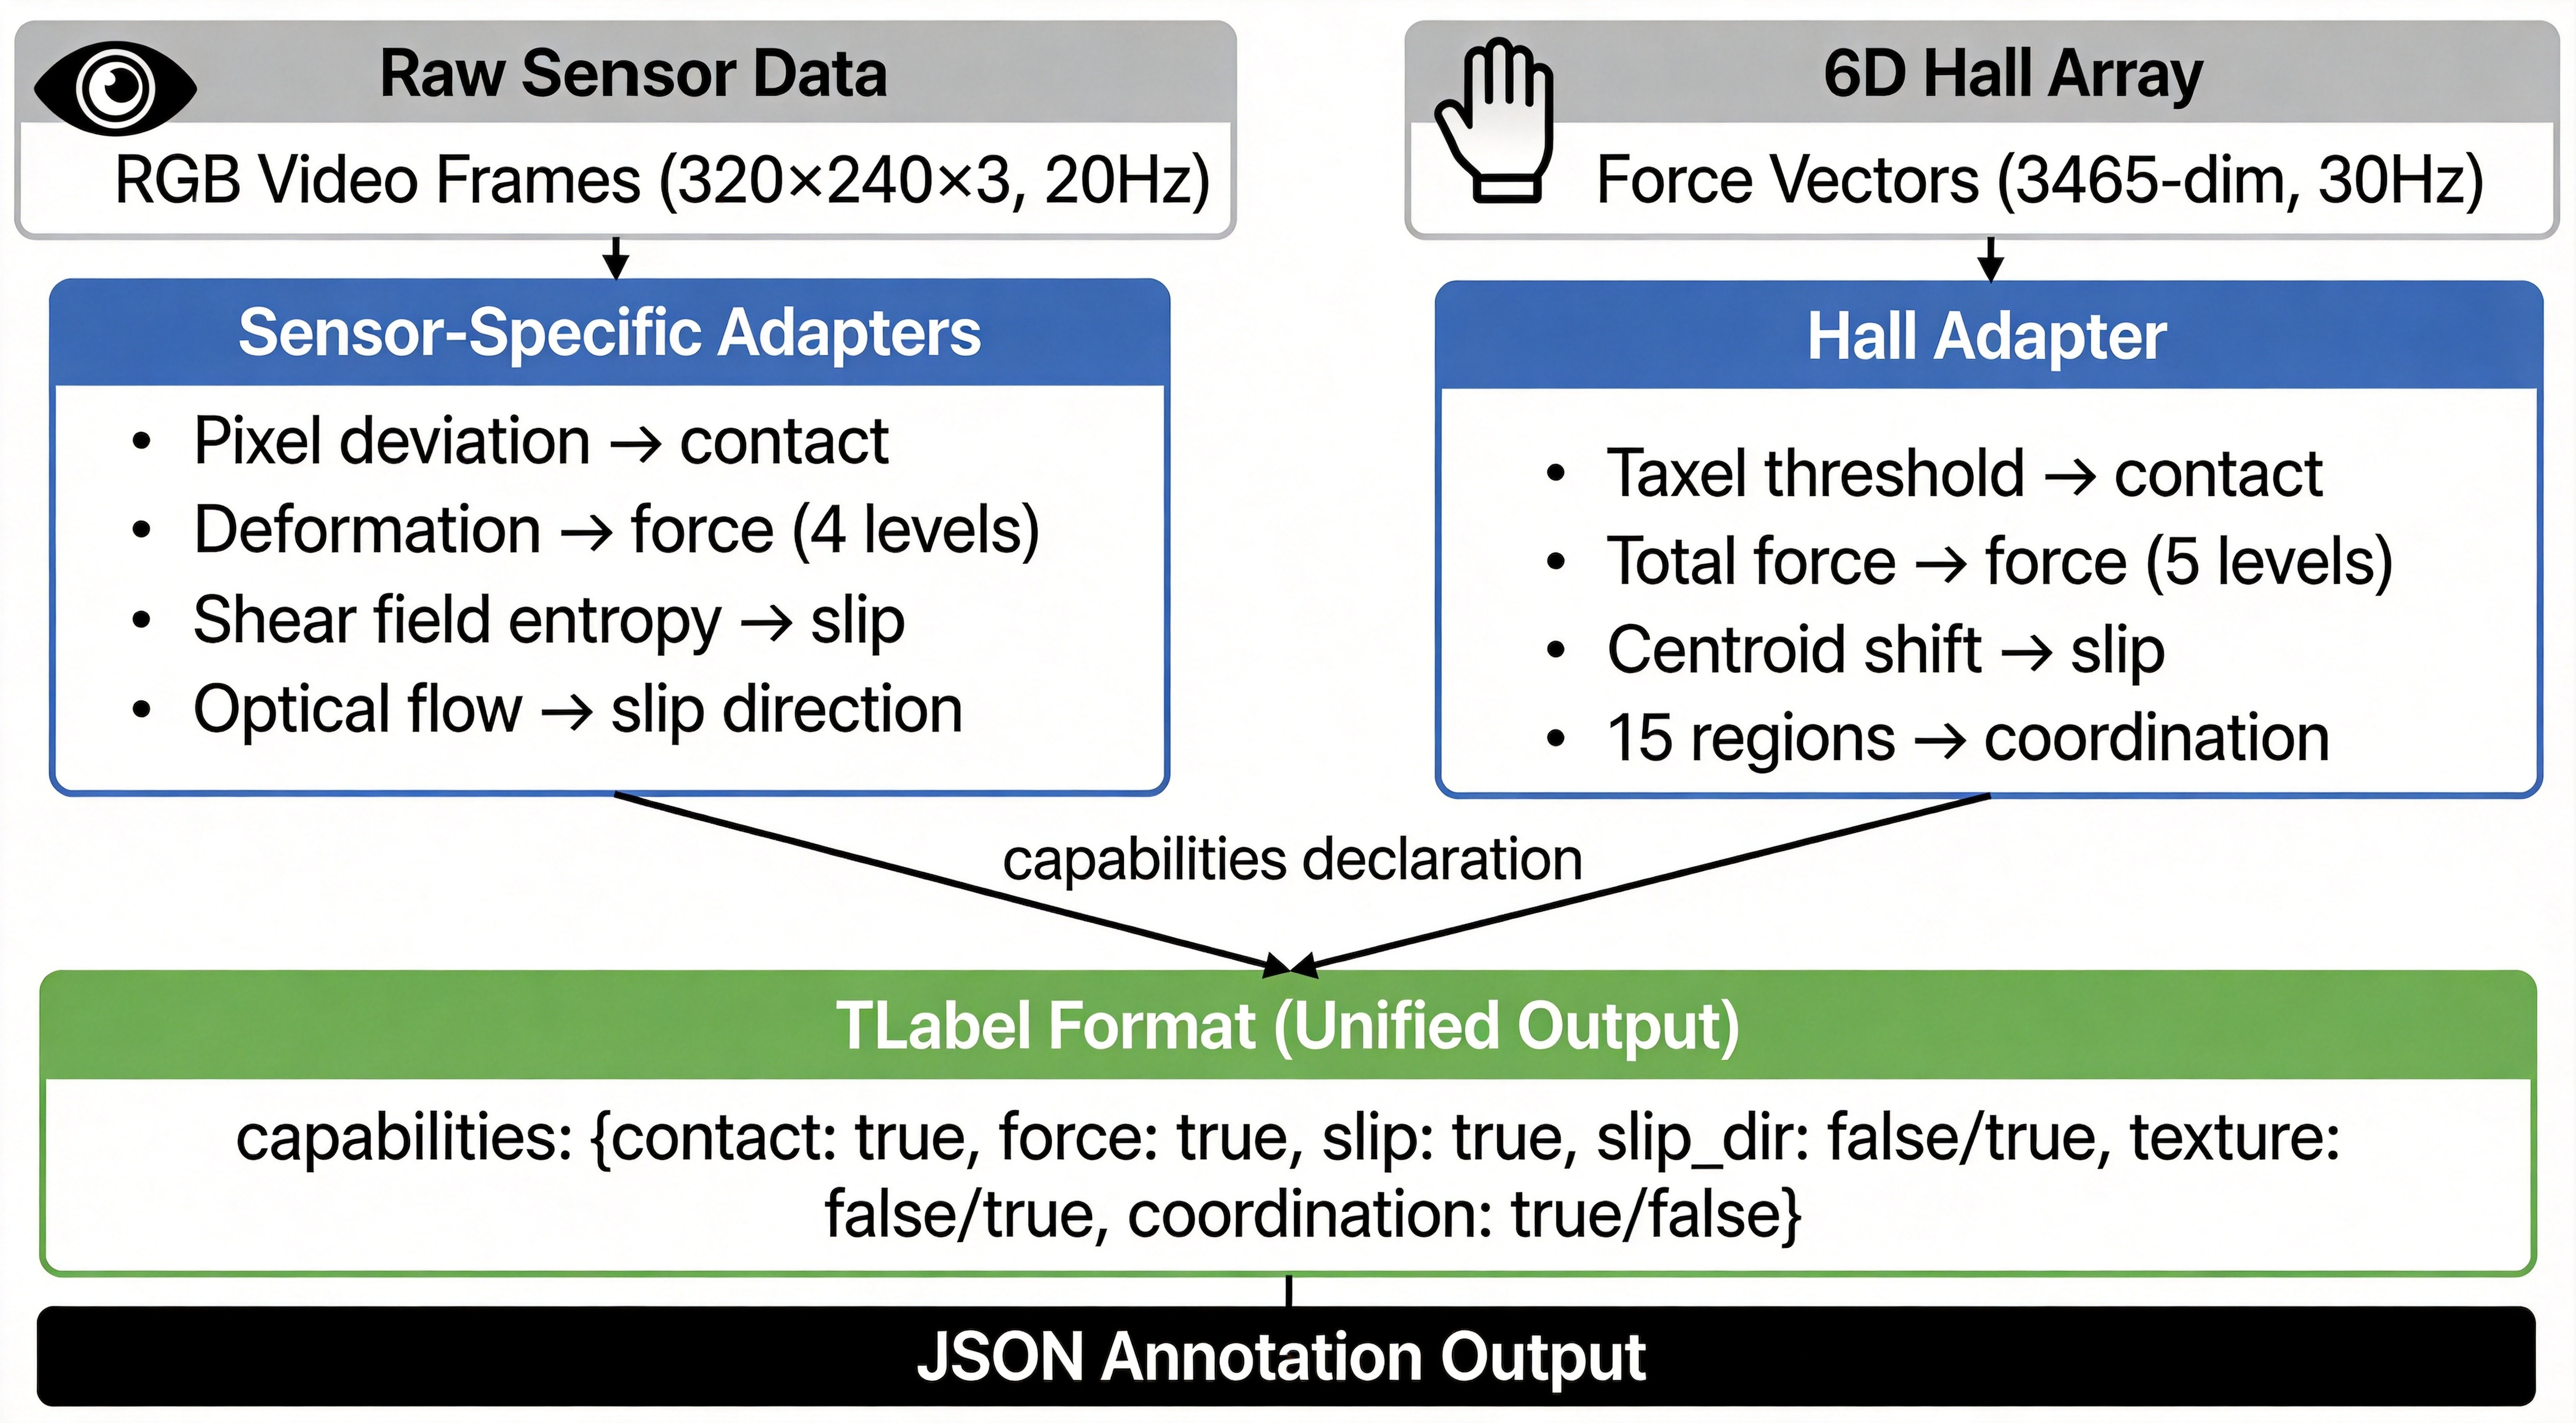
\includegraphics[width=\columnwidth]{tlabel-architecture-diagram.jpg}
\caption{TLabel architecture. Heterogeneous sensor data flows through sensor-specific adapters, each declaring capabilities, producing unified JSON output.}
\label{fig:architecture}
\end{figure}

The \texttt{capabilities} field is the critical innovation. It enables:
\begin{itemize}
\item \textbf{Consumers} to know which fields are reliable without examining the adapter code
\item \textbf{Fusion} of annotations from multiple sensors, using each sensor's strengths
\item \textbf{Graceful degradation} when a capability is unsupported (field is simply absent)
\end{itemize}

Table~\ref{tab:dimensions} summarizes the ten semantic dimensions.

\begin{table}[t]
\centering
\caption{Ten Semantic Dimensions of TLabel Format}
\label{tab:dimensions}
\begin{tabular}{cllc}
\toprule
\# & Dimension & Description & Scope \\
\midrule
1 & contact\_detection & Contact state classification & All \\
2 & force\_level & Multi-level force classification & All \\
3 & slip\_detection & Object slip detection & Most \\
4 & slip\_direction & Slip direction vector & GelSight \\
5 & texture & Surface texture classification & GelSight \\
6 & 3d\_shape & Local surface shape & GelSight \\
7 & shear\_force & Tangential force component & GelSight \\
8 & whole\_hand\_coord & Multi-region coordination & Arrays \\
9 & vibration & High-freq oscillation ($>$200Hz) & None \\
10 & temperature & Thermal contact info & None \\
\bottomrule
\end{tabular}
\end{table}

Of the 10 dimensions, 7 can be uniformly mapped across sensor types (dimensions 1--3, 8--10), while 3 are sensor-specific (GelSight: slip\_direction, texture, 3d\_shape; distributed arrays: whole\_hand\_coordination). The same semantic concept---e.g., ``contact detection''---is computed through fundamentally different physical processes (pixel deviation vs.\ force threshold), yet produces compatible output.

\section{Cross-Sensor Validation}

\subsection{Sensor Architectures}

We select two sensors that represent the two dominant tactile sensing paradigms. Table~\ref{tab:sensors} compares their characteristics.

\begin{table}[t]
\centering
\caption{Comparison of Validated Sensor Modalities}
\label{tab:sensors}
\begin{tabular}{lcc}
\toprule
& \textbf{Daimon} & \textbf{PaXini} \\
& \textbf{(GelSight)} & \textbf{(6D Hall)} \\
\midrule
Principle & Photometric stereo & 6-axis Hall array \\
Output & RGB frames (320$\times$240) & Float32 vectors \\
Spatial & 5 fingertips & 15 regions \\
Resolution & 76,800 px/sensor & 105--378 taxels \\
Force info & Indirect (deformation) & Direct (6-axis F/T) \\
Rate & $\sim$20 Hz & 30 Hz \\
Collection & Robot-mounted & Human glove \\
\bottomrule
\end{tabular}
\end{table}

These sensors differ in every dimension: sensing principle, output modality (image vs.\ number), spatial coverage (fingertip vs.\ whole hand), force representation (indirect vs.\ direct), and collection method (robot vs.\ human). This makes them an ideal test pair for cross-sensor generalization.

\subsection{Adapter Implementations}

Each adapter follows the same four-stage pipeline with sensor-specific implementations:

\textbf{Stage 1: Signal Analysis}
\begin{itemize}
\item GelSight: FFV1 video $\rightarrow$ ffmpeg decoding $\rightarrow$ per-frame numpy arrays
\item PaXini: HDF5 $\rightarrow$ h5py direct read $\rightarrow$ split by sensor\_lengths
\end{itemize}

\textbf{Stage 2: Baseline Computation}
\begin{itemize}
\item GelSight: Median of first N frames as no-contact reference
\item PaXini: Mean of first N frames per region
\end{itemize}

\textbf{Stage 3: Per-Frame Annotation}
\begin{itemize}
\item Contact detection: pixel deviation threshold (GelSight) / taxel value threshold (PaXini)
\item Force classification: deformation magnitude $\rightarrow$ 4 levels / total force $\rightarrow$ 5 levels
\item Slip detection: shear displacement field entropy (GelSight) / pressure centroid shift + force rate (PaXini)
\item Phase inference: velocity + contact $\rightarrow$ 7-stage FSM / velocity + force + trend $\rightarrow$ 8-stage FSM
\end{itemize}

\textbf{Stage 4: Quality Validation} --- 8-item self-consistency check (see Section~\ref{sec:validation}).

\subsection{Validation Methodology}
\label{sec:validation}

We define 8 self-consistency checks covering three severity levels:

\textbf{Hard errors (must be 0):}
\begin{enumerate}
\item \texttt{force\_none\_state\_active}: force=``none'' but contact$\neq$no\_contact
\item \texttt{force\_active\_state\_no\_contact}: force$\neq$``none'' but contact=no\_contact
\item \texttt{slip\_no\_contact}: slip\_detected but no contact
\end{enumerate}

\textbf{Soft anomalies (threshold-based):}
\begin{enumerate}\setcounter{enumi}{3}
\item \texttt{taxel0\_state\_active}: 0 active taxels but contact state $\neq$ no\_contact
\item \texttt{phase\_skip}: illegal phase transition (e.g., idle$\rightarrow$hold)
\item \texttt{first\_frame\_contact}: contact detected on first frame (baseline issue)
\item \texttt{region\_force\_contact\_mismatch}: contact state and mean\_force disagree
\item \texttt{hand\_state\_region\_mismatch}: hand-level state disagrees with region count
\end{enumerate}

\subsection{Results}

Table~\ref{tab:results} presents the validation results.

\begin{table}[t]
\centering
\caption{Cross-Sensor Validation Results}
\label{tab:results}
\begin{tabular}{lcc}
\toprule
\textbf{Metric} & \textbf{Daimon GelSight} & \textbf{PaXini 6D Hall} \\
\midrule
Episodes & 94 & 15 \\
Task types & 6 & 7 \\
Total observations & 370,516 & 219,510 \\
Hard errors & \textbf{0} & \textbf{0} \\
Anomaly rate & 2.91\% & 0.14\% \\
Grade & A & A \\
\bottomrule
\end{tabular}
\end{table}

Both sensors achieve zero hard errors, confirming that the core annotation logic is sound across modalities. The anomaly rate difference (2.91\% vs.\ 0.14\%) reflects different challenges: GelSight's boundary oscillation in high-precision tasks (peg\_in\_hole: 6.90\% anomaly rate) vs.\ PaXini's minimal soft anomalies (only phase transitions from human-like ``fragmented'' manipulation patterns).

\textbf{Soft anomaly analysis (PaXini):} All 301 soft anomalies are \texttt{phase\_skip} events caused by human-like fragmented manipulation---brief touch-release-re-touch sequences that violate strict FSM transitions but are physically reasonable. This is expected for wearable glove data and does not indicate annotation errors.

\subsection{Complementarity Analysis}

Table~\ref{tab:complementarity} summarizes the complementary strengths.

\begin{table}[t]
\centering
\caption{Sensor Complementarity Under TLabel}
\label{tab:complementarity}
\begin{tabular}{lcc}
\toprule
\textbf{Capability} & \textbf{GelSight} & \textbf{6D Hall} \\
\midrule
Surface detail & Slip dir, texture, 3D & --- \\
Force precision & --- & Direct 6-axis, linear \\
Spatial coverage & 5 fingertips & 15 regions, whole-hand \\
Task suitability & Precision tasks & Grasping tasks \\
\bottomrule
\end{tabular}
\end{table}

The two sensors are complementary: GelSight excels at surface-level phenomena while distributed arrays capture whole-hand coordination and direct force measurement. Under TLabel Format, both can contribute their strengths within a unified framework.

\section{Downstream Evaluation}

We validate annotation utility through three prediction experiments on Daimon data.

\subsection{Contact State Prediction}

Predict contact state $k$ steps ahead, comparing baseline features vs.\ baseline + TLabel annotation labels.

\begin{table}[t]
\centering
\caption{Contact State Prediction Across Horizons}
\label{tab:contact_pred}
\begin{tabular}{lccc}
\toprule
\textbf{Horizon} & \textbf{Baseline F1} & \textbf{+TLabel F1} & \textbf{Gain} \\
\midrule
$k$=1 & 0.903 & 0.904 & +0.10\% \\
$k$=3 & 0.869 & 0.865 & $-$0.38\% \\
$k$=5 & 0.818 & 0.834 & +1.63\%* \\
\bottomrule
\end{tabular}
\end{table}

Annotations provide the most benefit for longer-horizon prediction, where semantic priors compensate for signal decay (*$p<0.001$, proportion test).

\subsection{Cross-Scenario Generalization}

Table~\ref{tab:generalization} shows leave-one-scenario-out results.

\begin{table}[t]
\centering
\caption{Cross-Scenario Generalization (Leave-One-Out)}
\label{tab:generalization}
\begin{tabular}{lccc}
\toprule
\textbf{Test Scenario} & \textbf{Baseline} & \textbf{+TLabel} & \textbf{Gain} \\
\midrule
Peg insertion & 0.856 & 1.000 & +14.4\% \\
Block insertion & 0.854 & 1.000 & +14.6\% \\
Whiteboard wiping & 0.881 & 1.000 & +11.9\% \\
Tube handling & 0.963 & 1.000 & +3.7\% \\
Wrench storage & 0.985 & 0.999 & +1.3\% \\
Plug insertion & 0.983 & 0.998 & +1.5\% \\
\midrule
\textbf{Average} & \textbf{0.920} & \textbf{0.999} & \textbf{+7.9\%} \\
\bottomrule
\end{tabular}
\end{table}

The largest gains occur in the hardest scenarios, confirming that annotations serve as semantic priors for cross-domain transfer. The improvement is statistically significant (paired t-test, $t=3.04$, $p=0.029$, Cohen's $d=1.24$).

\subsection{Slip Risk Prediction}

\begin{table}[t]
\centering
\caption{Slip Risk Prediction Results}
\label{tab:slip_pred}
\begin{tabular}{lcc}
\toprule
\textbf{Model} & \textbf{Accuracy} & \textbf{F1 (high-risk)} \\
\midrule
Baseline (no slip label) & 0.970 & 0.896 \\
+TLabel slip annotation & 0.999 & 0.999 \\
\textbf{Gain} & \textbf{+2.9\%} & \textbf{+10.4\%} \\
\bottomrule
\end{tabular}
\end{table}

Slip annotations dramatically reduce missed detections in the high-risk class ($p<0.001$, proportion test), which is critical for safety-sensitive manipulation.

\section{Discussion}

\subsection{Why Cross-Sensor Unification Works}

The feasibility of cross-sensor annotation rests on a key observation: while raw tactile signals are fundamentally different across sensor types (images vs.\ force vectors), the \emph{semantic phenomena} they capture---contact, force, slip, grasp phases---are shared. TLabel Format operates at this semantic level, allowing each sensor to contribute its unique measurement modality while producing compatible output.

\subsection{Sensor Complementarity}

Our results show that the two sensors are not competitors but complements. This has practical implications:
\begin{itemize}
\item \textbf{For data collection:} Choose sensors based on task requirements---GelSight for surface inspection, distributed arrays for whole-hand manipulation
\item \textbf{For annotation reuse:} The PaXini adapter can be directly reused for other flexible e-skin vendors that use similar distributed array architectures
\item \textbf{For data fusion:} TLabel annotations from different sensors can be merged, combining surface detail with whole-hand coordination
\end{itemize}

\subsection{Limitations}

\begin{itemize}
\item \textbf{Validation scale:} 15 PaXini episodes provide proof-of-concept but insufficient for statistical confidence in parameter tuning
\item \textbf{Slip detection quality:} PaXini's slip detection is indirect (pressure centroid shift) without academic validation, unlike GelSight's entropy-based method
\item \textbf{Phase FSM design:} Human-collected data shows fragmented manipulation patterns that violate strict FSM assumptions; future work should incorporate probabilistic phase models
\item \textbf{Sensor coverage:} Only two sensor types validated; extending to DIGIT, BioTac, 6-axis F/T sensors remains future work
\end{itemize}

\subsection{Future Work}

\begin{itemize}
\item Multi-sensor $\times$ multi-task cross-validation matrix for conference submission
\item Probabilistic phase modeling to handle fragmented manipulation
\item Additional sensor adapters (DIGIT, BioTac, F/T sensors)
\item Public benchmark and annotation challenge
\end{itemize}

\section{Conclusion}

We presented TLabel Format, the first cross-sensor unified annotation framework for tactile manipulation data. By operating at the semantic level through capability declarations, TLabel enables heterogeneous tactile sensors to produce compatible annotations while preserving their unique strengths. Validated on two fundamentally different sensor modalities---vision-based GelSight and distributed 6D Hall-effect arrays---TLabel achieves zero hard errors across 109 episodes and 590K+ observations. Downstream experiments confirm that annotations provide measurable benefits: +7.93\% cross-scenario generalization and +10.35\% slip-risk F1. Our results demonstrate that cross-sensor tactile annotation is not only feasible but preserves the complementary strengths of different sensing modalities, paving the way toward standardized tactile data annotation in robotics.

\bibliographystyle{IEEEtran}
\begin{thebibliography}{17}

\bibitem{daimon2026}
Daimon-Infinity: Large-Scale Vision-Tactile-Language-Action Dataset. ModelScope, 2026. \url{https://www.modelscope.cn/datasets/daimonrobotics/Daimon-Infinity}

\bibitem{zhao2024t3}
Y.~Zhao et al., ``Transferable Tactile Transformers for Cross-Sensor Tactile Representation Learning,'' in \emph{Proc.\ ICRA}, 2024. arXiv:2406.13640.

\bibitem{feng2025anytouch}
Y.~Feng et al., ``AnyTouch: Learning Unified Manipulation Representation via Multi-Task Tactile Instruction Tuning,'' in \emph{Proc.\ ICLR}, 2025. arXiv:2502.12191.

\bibitem{opentouch2025}
OpenTouch: First-Person Whole-Hand Tactile Dataset. arXiv:2512.16842, 2025.

\bibitem{sitr2025}
SITR: Sensor-Invariant Tactile Representation via Physically-Based Rendering. arXiv:2502.19638, 2025.

\bibitem{tlvcore2025}
TLV-CoRe: Tactile-Language-Vision Cross-Modal Contrastive Representation. in \emph{Proc.\ AAAI}, 2025.

\bibitem{dong2017gelsight}
S.~Dong et al., ``GelSight and GelSlim: High-Resolution Tactile Sensors for Robot Manipulation,'' in \emph{Proc.\ ICRA}, 2017.

\bibitem{hu2024slip}
Z.~Hu et al., ``Slip Detection via Contact Force Field Entropy Analysis with GelSight Mini,'' 2024.

\bibitem{feelanyforce2025}
A.~Shahidzadeh et al., ``FeelAnyForce: Force Estimation from Vision-Based Tactile Images,'' in \emph{Proc.\ ICRA}, 2025. \url{http://prg.cs.umd.edu/FeelAnyForce}

\bibitem{feats2024}
FEATS: Force Estimation with FEA Training for Vision-Based Tactile Sensors. arXiv:2411.03315, 2024.

\bibitem{paxini2025}
PaXini OmniSharingDB: Multi-Task Tactile Manipulation Dataset with 6D Hall-Effect Glove. HuggingFace, 2025.

\bibitem{sparsh2024}
C.~Higuera et al., ``Sparsh: Self-Supervised Touch Representations for Vision-Based Tactile Sensing,'' in \emph{Proc.\ NeurIPS}, 2024. arXiv:2410.24090.

\bibitem{openx2024}
Open X-Embodiment: Robotic Learning Datasets and RT-X Models. Google DeepMind, 2024. \url{https://robotics-transformer-x.github.io}

\bibitem{lerobot2024}
LeRobot: An Open-Source Library for End-to-End Robot Learning. Hugging Face, 2024. in \emph{Proc.\ ICLR}, 2026.

\bibitem{yuan2017gelsight}
W.~Yuan et al., ``GelSight: High-Resolution Robot Tactile Sensors for Estimating Geometry and Force,'' \emph{Sensors}, 2017.

\bibitem{tacquad2025}
TacQuad: Paired Multi-Sensor Multi-Modal Tactile Dataset. in \emph{Proc.\ ICLR}, 2025.

\bibitem{fota2024}
FoTa: Foundation Tactile Dataset for Multi-Sensor Pre-Training. 2024.

\end{thebibliography}

\end{document}
